\documentclass[10pt,conference]{IEEEtran}

\usepackage{cite}
\usepackage{chngcntr}


\ifCLASSINFOpdf
   \usepackage[pdftex]{graphicx}
   \graphicspath{{figs/}}
   \DeclareGraphicsExtensions{.pdf,.jpeg,.png}
\else
   \usepackage[dvips]{graphicx}
   \graphicspath{{../figs/}}
   \DeclareGraphicsExtensions{.eps}
\fi

\usepackage[cmex10]{amsmath}
\interdisplaylinepenalty=2500
\usepackage{amsthm}
\newtheorem{definition}{Definition}
\usepackage{algorithmic}
\usepackage{array}
\usepackage{subcaption}
\usepackage{url}

\usepackage[T1]{fontenc}
\usepackage[utf8]{inputenc}


\usepackage[margin=1in]{geometry} 
\usepackage{amsmath,amsthm,amssymb}
\usepackage{graphicx}
\usepackage{graphics}
\usepackage{float}		
\usepackage{times}		

\usepackage{enumitem}
% \usepackage{enumerate}
\usepackage{pbox}
\usepackage{amsmath}		% so that equation* works
\usepackage{pgfplots}
\usepackage{multirow}
\usepackage{listings}
\usepackage{url}

\usepackage{xcolor}
\usepackage[colorlinks = true,
            linkcolor = blue,
            urlcolor  = blue,
            citecolor = blue,
            anchorcolor = blue]{hyperref}

% corrija hifenação aqui
%\hyphenation{op-tical net-works semi-conduc-tor}

\begin{document}
\title{Applied Machine Learning: Project 3 \\ Image Classification}





\author{Chengkai Zhu \\ (260775967) \\ \textit{\normalsize{chengkai.zhu@mail.mcgill.ca}}
\and
\ Aman Garg \\ (260744367) \\ 
\textit{\normalsize{aman.garg@mail.mcgill.ca}}
\and
\ Meixue Liu \\ (260748593) \\ 
\textit{\normalsize{meixue.liu@mail.mcgill.ca}}}






\maketitle

\IEEEpeerreviewmaketitle

\textbf{Team Name: CAM CAM CAM}

Codes:\url{https://github.com/saberkid/Modified-MNIST-Classifier}

\section{Introduction}
% Introduction: briefly describe the problem and summarize your approach (1 paragraph).
The automatic classification of text in images has witnessed a booming interest in the last 25 years, due to the increased availability of documents in digital format and the ensuing needs of processing them to speed up information recognition and retrieval. Moreover, the increasing popularity of multimedia and digital devices has elevated the importance of content-based image retrieval system. Text data presented in images play a significant role in the retrieval system because they contain plenty of useful information for automatic annotation, indexing, and structuring of images. This extraction involves localization, detection, enhancement and recognition of the text. There are various challenges like variations in text due to differences in font, size, contrast, orientation, complicated background and etc. Therefore, the needs of the automatic system of text detection and extraction from the images have increased in recent years.

This report discusses and compares various approaches of image classification that fall within the machine learning paradigm. We experimented and evaluated the accuracy and error for different classifiers: Logistic Regression, Support Vector Machines(SVM), Neural Network, Convolutional Neural Network (CNN) and Ensemble Method.

\section{Related work}
% Related work: previous literature related to text classification problem (max. ½ page).

Back to 1990, LeCun, Yann et al.\cite{lecun1990handwritten} researched on the implementation of back-propagation networks to hand-written digit recognition, and successfully applied it to a commercial digital signal processing hardware. Compared with its previous works that applied an elaborate feature extraction and hand-chosen constants in each connected layer in a neural network, this study built a multi-layer network with adaptive connections and minimal preprocessing. By training with back-propagation, the network designed for hand-written digit recognition achieved a 1\% error rate within a shorter learning time. 

Nowadays, there has been lots of research on developing a better model for image analysis and classification. Fernando, Chrisantha et al.\cite{fernando2017pathnet} brought a state-of-art model, PathNet, to speed up learning in MNIST classification task. Different from deep learning algorithm that learns bias and weights of a network by gradient descent, PathNet makes choice of a subset of parameters need to be trained. In terms of classification loss, the state of art solution is brought by Wan, Li et al. Their implementation using DropConnect achieved a 0.21\% error rate in MNIST classification task\cite{wan2013regularization}.

\section{Problem representation}
The training set consists of 50,000 8bit-greyscale images of size 64x64. There is a unique label for each of the examples, representing the result from the mathematical operation of the two digits in the image ( result for "a"/"A" is the sum of the two digits and result for "m"/"M" is the product of the two digits ). The total number of unique classes are 40 ( [0, 1, 2, 3, 4, 5, 6, 7, 8, 9, 10, 11, 12, 13, 14, 15, 16, 17, 18, 20, 21, 24, 25, 27, 28, 30, 32, 35, 36, 40, 42, 45, 48, 49, 54, 56, 63, 64, 72, 81] ). The test set consists of 10,000 images in the same format.

The aim of this project is to develop a machine learning model which could predict the result of the mathematical operation based on the character and digits in each image. The number of examples per class is non-uniform, thus we assumed that the class proportions are similar for the training and test set. 

% o Problem representation: data pre-processing methods, feature design/selection methods.
\subsection{Pre-Processing Dataset}

Since there is lots of background noise in the dataset, pre-processing the raw data would allow us to experiment different models separately with a raw and a cleaner dataset.

To pre-process the dataset, first, image binarization was implemented to segment each image into background and foreground containing digits and letter (Fig.\ref{bin}). Image Binarization is the conversion of a color-scaled image into a bi-level image \cite{trier1995evaluation}. Image pixels were separated into dual collection of pixels, i.e. black and white. Binarization was applied to our dataset in order to obtain clear images to easily retrieve the digits in each image. The threshold used for binarization was set to 190. Moreover, two files for training (one with image dataset and other with the labels) were merged into one.

\begin{figure}
  \centering
  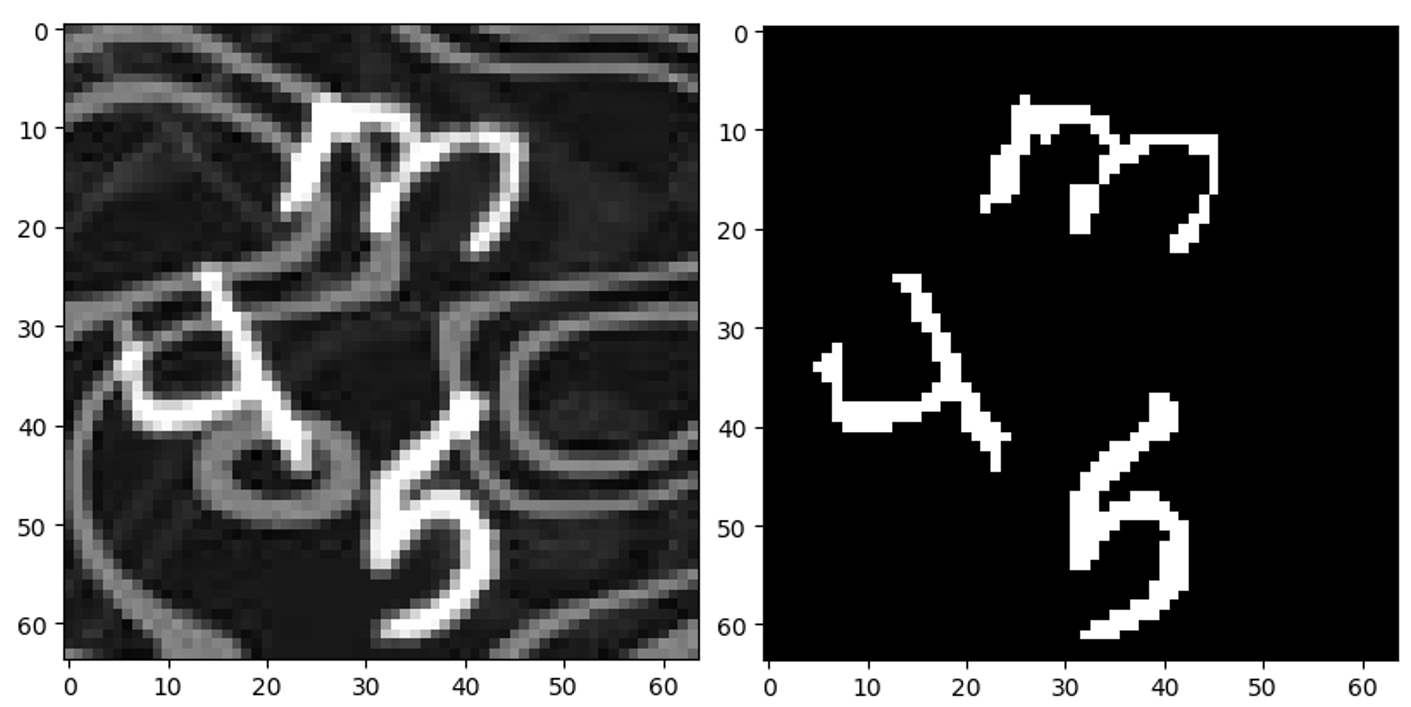
\includegraphics[width = 0.6\linewidth]{binary}
  \caption{Binarization}
  \label{bin}
\end{figure}
%spelling error, not figura 1
For a classification task, label 'y' is usually processed by one-hot encoder in advance. In this case, the number of categorical features is identical to the number of classes for y. Consequently, each label 'y' was encoded into a 1*40 vector during the pre-processing phase.

% For citing: ~\cite{itseez2015opencv}.

\subsection{Validation data}
To evaluate algorithms that we chose, we constructed a validation dataset from the training dataset. The validation data is 20\% of the actual training set size. It was made sure that the number of validation examples in each output class was proportionally extracted according to its size in the original training dataset. Finally, the new training data was shuffled so that it would not get different distributions when constructing models with batch-wise datasets.

%\subsection{Cluster Resources}

\section{Algorithm selection and implementation}

\subsection{Algorithm 1: Logistic Regression}
We chose Logistic Regression as our baseline linear classification algorithm. The sklearn module was used to construct the LR \cite{pedregosa2011scikit}. 

\subsection{Algorithm 2: Support Vector Machines}
Support Vector Machine (Linear) was also used as the second baseline classification algorithm. The sklearn module was used to construct the SVM\cite{pedregosa2011scikit}. 

\subsection{Algorithm 3: Neural Network}
Neural Network (NN) is one of the most popular approaches to capture the non-linear relation existing in the dataset. 

We implemented a feed-forward neural network from scratch to classify the modified MNIST images. There are three layers in our home-made NN: an input layer, a hidden layer and an output layer. And we applied softmax function to the output layer to make it a multi-class classifier. After figuring out the basic architecture of our NN, we initiated weighs by assigning a random value multiplied by a standard variable (0.01 by default). Then, cross-entropy cost function  was applied to compute the loss, which is a way to avoid learning slowdown issue caused by  $\sigma$'(z) term within the implementation of quadratic cost in NN. Cross-entropy error (CE) is defined as the following equation:

\begin{equation}\label{eq1}
H_{y^{'}}(y)=-\sum_{i}y_{i}^{'}log(y_{i})
\end{equation}

To boost training speed, we grouped training data into batches and averaged the cross-entropy error generated from each batch, dividing CE error by batch size. 

For the sake of minimizing the cross-entropy cost, we trained the model by back propagation. We implemented a backward function for each layer in which the error of weights and bias ($dW$ and $dB$) is defined in the direction of gradient. And during the training phase for each batch, we updated weights in each layer by subtracting the error multiplied by learning rate.

\begin{figure}[!tbhp]
\centering
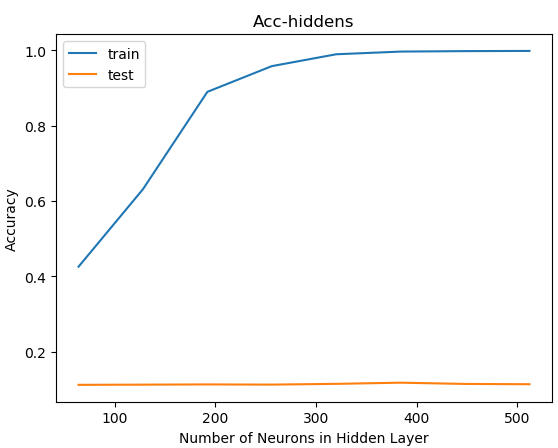
\includegraphics[width = 0.6\linewidth]{hiddens}
\caption{Accuracy vs Hiddens}
\label{fig:hidden}
\end{figure}

\begin{figure}[!tbhp]
\centering
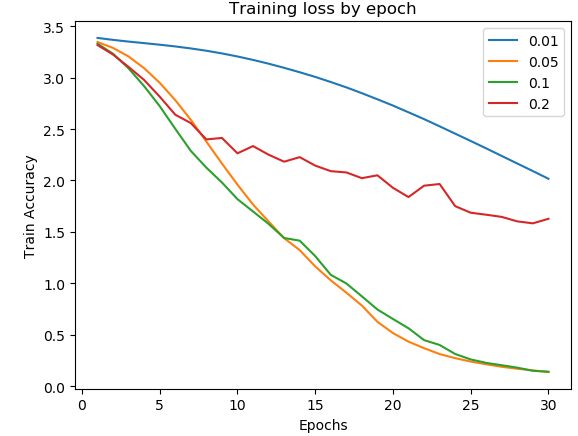
\includegraphics[width = 0.6\linewidth]{lr}
\caption{Training Accuracy with different learning rates}
\label{fig:lr}
\end{figure}
Using cross validation, we varied the number of neurons in hidden layers to see if it influences the performance of the network. Fig.\ref{fig:hidden} shows the averaged training and validation accuracy for different sizes of hidden layers. With the same learning rate and epochs, we could interpret from the training accuracy curve that we have a more precise model with the growth of hidden neurons. On the other hand, the number of neurons in hidden layers barely affects the averaged validation accuracy which indicates a two-layer network may not a model with sufficient learning capacity given the proposed image classification task.

We further verified our implementation by tuning learning rate and plotting the variance of training accuracy by each epoch, Fig.\ref{fig:lr}. According to the figure, training with learning rate of 0.05 and 0.1 would lead to faster convergence. With a learning rate of 0.2, we could see a unstable loss curve which is probably due to the theorem that large learning rate would induce oscillation of gradient descent\cite{jacobs1988increased}. 

\subsection{Algorithm 4: Convolutional Neural Networks}
Convolutional neural networks(CNN) are hierarchical networks where connection between neurons resembles that of visual cortex \cite{matsugu2003subject}. The implementation of CNN differs in how convolutional and sub-sampling layers are connected, and in how the nets are trained. In this work, the architecture of CNN is designed as a fully convolutional hierarchical model which largely resembles the layout of VGG16\cite{simonyan2014very}.

The architecture of our network is summarized in Fig.\ref{fig:CNN}. It contains 16 learned layers, 10 convultional and 3 maxpooling functioned as feature extraction layers, and 3 fully connected (Dense) as multi-class classifier.


\begin{figure}[!tbhp]
	\centering
	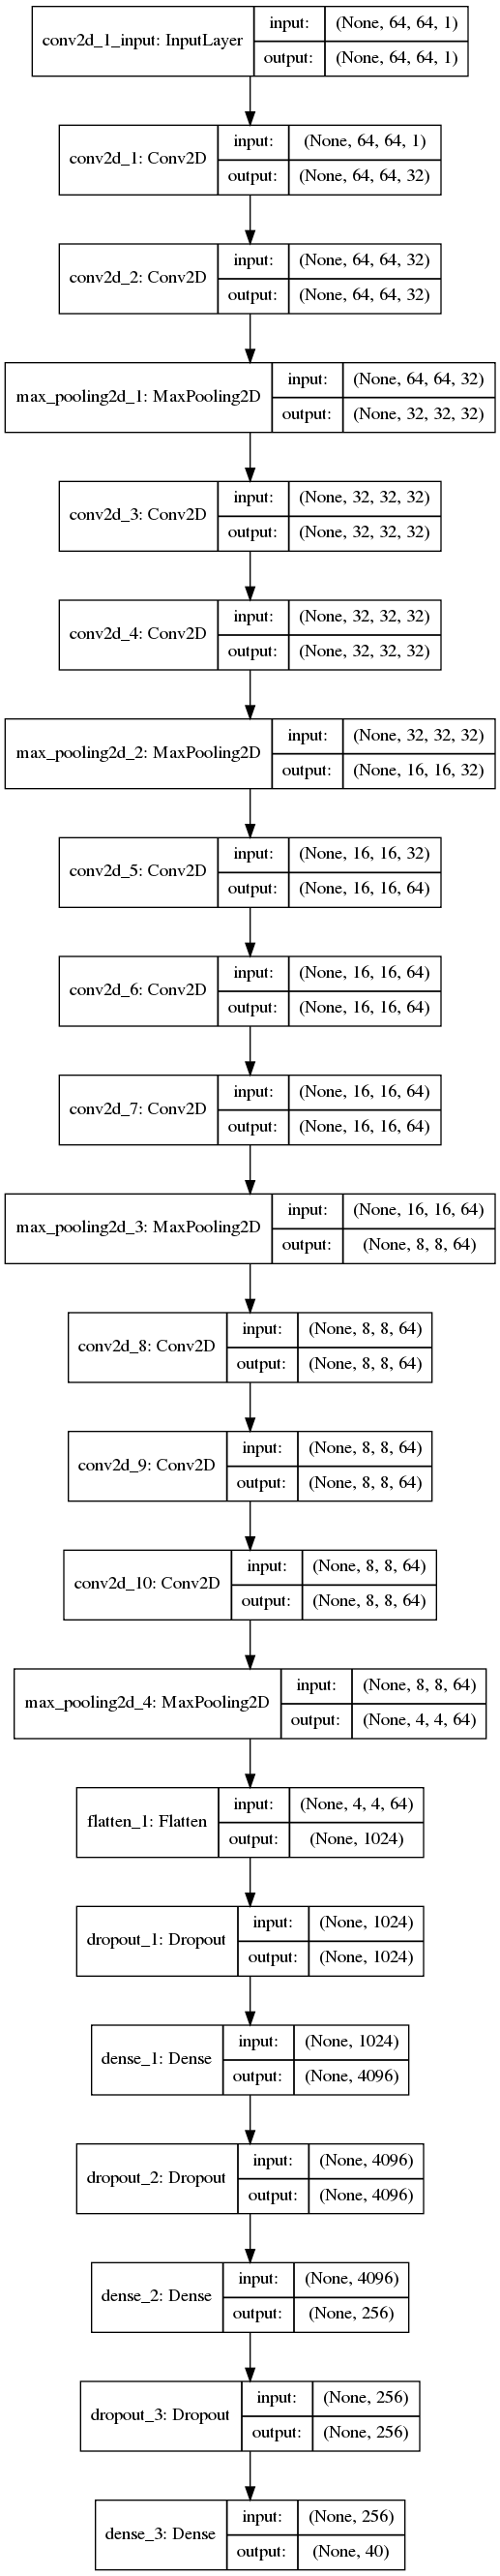
\includegraphics[width = 0.55\linewidth]{model3.png}
	\caption{CNN Architecture}
	\label{fig:CNN}
\end{figure}

Typically, a convolutianal layer is parametrized by the number of filters, filter sizes and stride. Letting $W$ to be the size of image, $K$ to be the size of filter and $S$ to be the stride, without padding to the image matrix, the output dimension $O$ could be calculated as:
\begin{equation}\label{eq2}
O=\frac{(W-K)}{S}+1
\end{equation}

\begin{figure}[!tbhp]
\centering
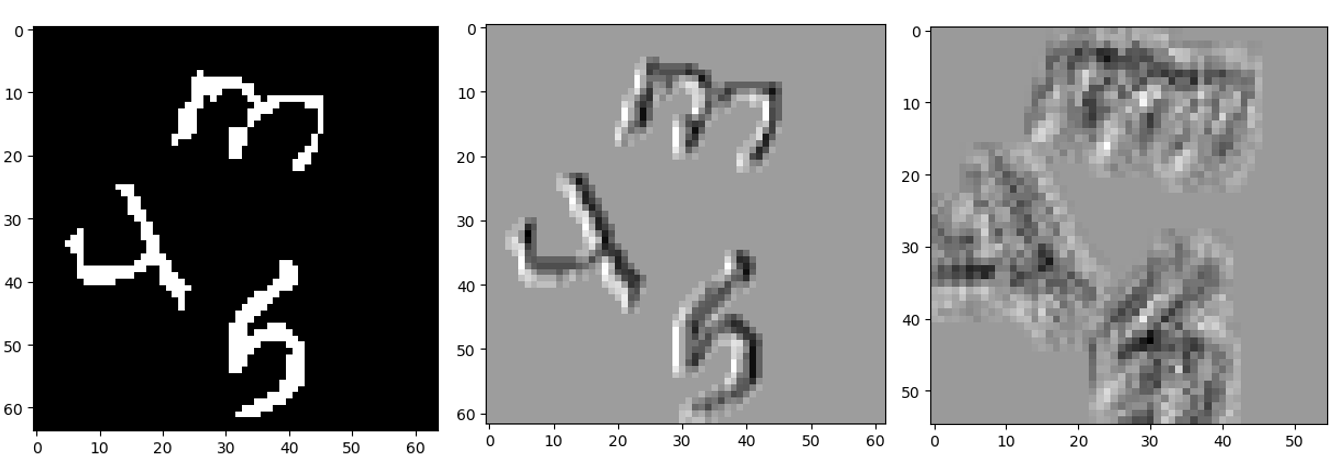
\includegraphics[width = 0.6\linewidth]{filter_size.jpg}
\caption{Original, 3x3 filter and 10x10 filter}
\label{fig:filter}
\end{figure}

From Fig.\ref{fig:filter}, we could see what happens to a input image convolving with a 3x3 and 10x10 filter respectively. A larger size of kernel leads to a more blurred edges and would extract a more general feature while the smaller size would focus more on features in a near neighbor.

\begin{figure}[!tbhp]
\centering
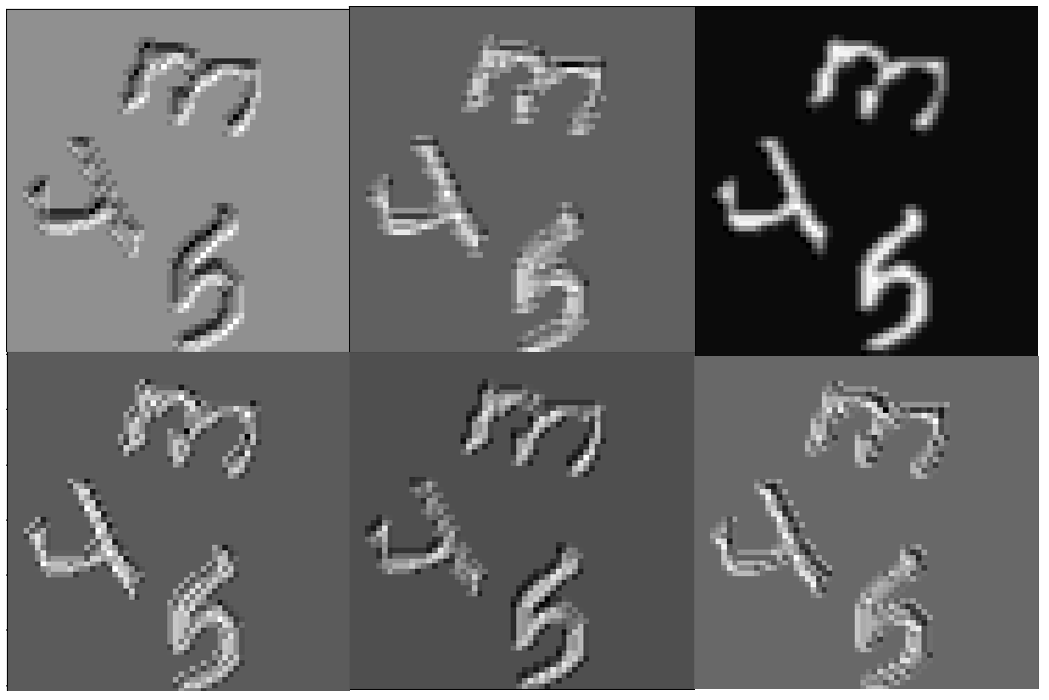
\includegraphics[width = 0.5\linewidth]{filters.jpg}
\caption{Images through 6 convolutional filters with the size of 3x3}
\label{fig:diff_filter}
\end{figure}

The number of filters N determines how many kernels are convolved with the input matrix (see Figure \ref{fig:diff_filter}). The output size of convolutional layer was set as (O, O, 1, N) while O was defined in Equation (\ref{eq2}). 

The activation function placed after the convolutional layer is usually selected between $f(x)=tanh(x)$ and $f(x)=max(0,x)$. The latter one is called Rectified Linear Units (ReLU). In terms of training time, we found the one using ReLU function was much faster.

A sub-sampling layer was placed following the convolutional layer and its activation. Sub-sampling layer is usually implemented as a max-pooling layer (Figure \ref{fig:max}). According to prior work, max-pooling is outstanding in that it leads to faster convergence and a better generalization of the model\cite{scherer2010evaluation}.The output dimension of max-pooling layer is the size of input divided by the pooling size (i.e 2x2 in our model).


\begin{figure}[!tbhp]
\centering
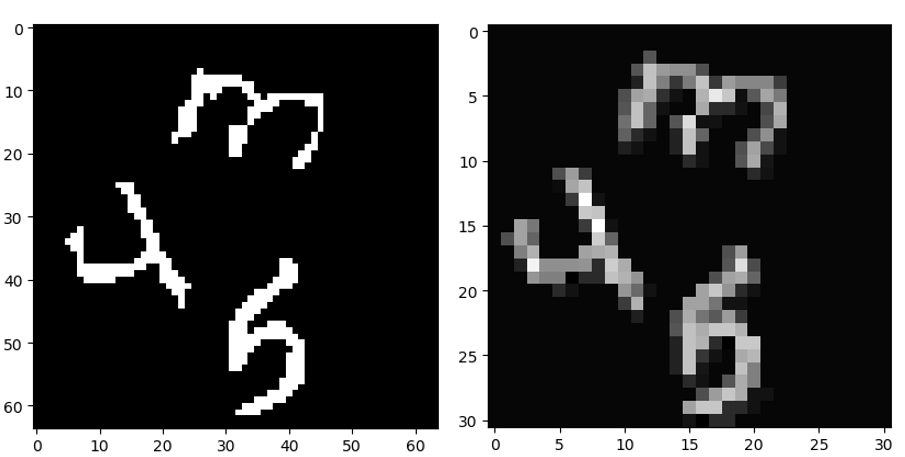
\includegraphics[width = 0.5\linewidth]{maxpooling.jpg}
\caption{Image through Maxpooling}
\label{fig:max}
\end{figure}


\begin{table*}[!tbhp]
\resizebox{\linewidth}{!}{
%\begin{tabular}{|c|c|c|c|}
\begin{tabular}{|l|l|l|l|}
\hline
Algorithm & Training Accuracy & Validation Accuracy & Test Accuracy (Kaggle)\\
\hline
Logistic Regression & 0.086 & 0.091 & 0.055\\
SVM & 0.059 & 0.035 & 0.028\\
Neural Network (2-layer) &0.997 & 0.117 & 0.108\\
CNN & 0.998 & 0.986 & 0.952\\
CNN with batch normalization & 0.994 & 0.983 & 0.949\\
Ensemble Method & - & - & 0.976\\
\hline
\end{tabular}
}
\caption{Accuracy achieved by various algorithms}
\label{table:accr}
\end{table*}


\subsection{Algorithm 5: Ensemble Methods}
In addition, we used ensemble learning method to reduce the variance in the classification problem. The mode was calculated to combine the results from various Neural Neural methods using majority voting. 

There were many cases, making impossible to calculate the mode. Thus, most accurate algorithm was set as default value, in case of no specific mode for some data points. Again new mode was calculated in similar way for the results with previous mode as default value. We obtained maximum accuracy on test dataset (more than 96\%) by using this method.

The Fig.\ref{fig:cross} shows the cross plot between test results of Ensemble method and CNN. It depicts the similarity and difference between two methods that classified the images into 40 classes.

% add figure
\begin{figure}[!tbhp]
\centering
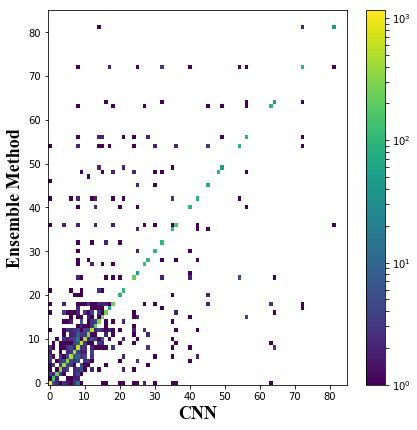
\includegraphics[width = 0.6\linewidth]{histo.png}
\caption{Comparison of Ensemble Method and CNN. The frequency count for each class is represented as a colorbar that is on a logarithmic scale}
\label{fig:cross}
\end{figure}

\section{Testing and Validation}
% Testing and validation: detailed analysis of your results, outside of Kaggle.
\subsection{Computing Resources}
Copper Cluster (by SHARCNET) was used for running the codes. Copper is a contributed cluster (with 4 non-contributed nodes), and the contributors have a higher priority for jobs.

\subsection{Results}
In terms of accuracy on training and validation set, the performance of each applied algorithms is shown in Table~\ref{table:accr}. Specifically, the two-layer neural network has 4096 hidden neurons and was trained after 30 epochs with learning rate 0.05. CNN implementation was trained using optimizer 'Adam'\cite{kingma2014adam} with a batch size of 128. 

Fig.\ref{fig:acc} shows the model accuracy on training and validation datasets. From the plot, we can see that the model could probably be trained more as the trend for accuracy on both datasets was still rising for the last few epochs. We can also see that the model has not yet over-learned the training dataset, showing comparable skill on both datasets.Fig.\ref{fig:loss} shows model loss on training and validation datasets. From the plot of loss, we conclude that the model has comparable performance on both training and validation datasets. If these parallel plots start to depart consistently, it might be a sign to stop training at an earlier epoch. Thus after 30 epochs, we saved the weights and retrained the model for 70 more epochs with saved weights and this time, batch size was changed from 128 to 1024. Changing batch size increased the training accuracy to 0.998 and Kaggle accuracy to 0.976 (after ensemble method).

\begin{figure}[!tbhp]
\centering
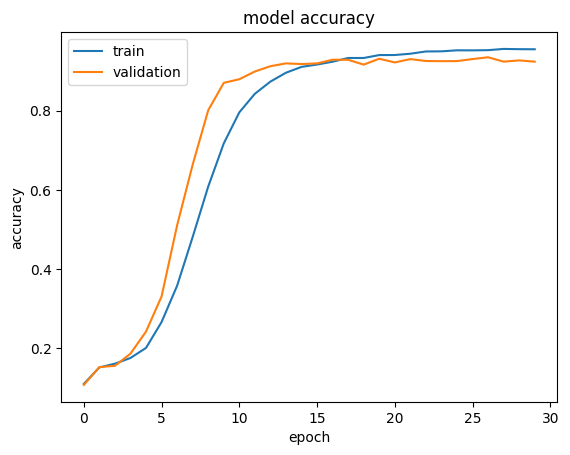
\includegraphics[width = 0.77\linewidth]{acc.png}
\caption{Plot of Model Accuracy on Train and Validation Datasets}
\label{fig:acc}
\end{figure}



\section{Discussion}
% o Discussion: pros/cons of your approach & methodology.
At the stage of network tunning, we found multiple useful techniques which accelerated the convergence of NN and led to a model with better performance.
\subsection{Dropout}

The most prominent method we implemented is to add more dropout into our model. Combining the predictions from multiple models is a very useful way to reduce test errors. In terms of neural networks, adding dropout is an efficient way to combine several models.\cite{hinton2012improving} With dropout $d$ added, a certain percentage of neurons turned off in the phase of forward propagation with probability $d$. At test time, we used all neurons through the feed-forward process. By adding more dropout, we reduced overfitting by ensembling predictive distributions produced from many dropout networks.

In Fig.\ref{fig:accd} and \ref{fig:lossd}, we presented the training and validation accuracy and loss for models with the exact same architecture and parameters except the insertion of dropout. We found that training was accelerated but the model suffered from substantial overfitting without dropout inserted. 

\begin{figure}[!tbhp]
\centering
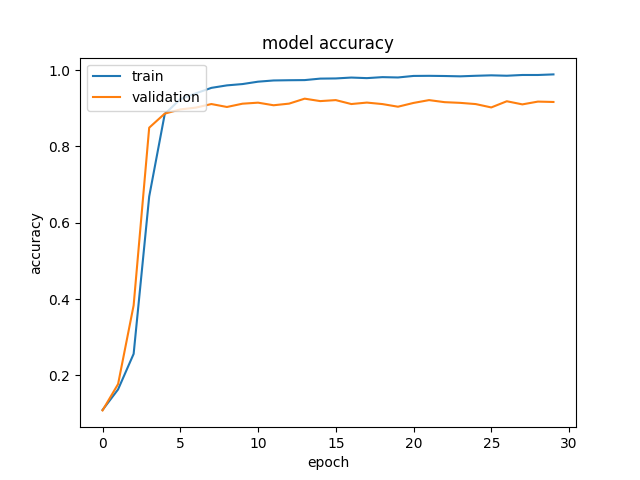
\includegraphics[width = 0.85\linewidth]{acc_d.png}
\caption{Plot of Model Accuracy on Train and Validation Datasets after removing the dropouts}
\label{fig:accd}
\end{figure}

\subsection{Data Augmentation}
Another way we tried to combat overfitting is by implementing data augmentation. Data augmentation is a widely-used approach in few-shot learning\cite{fei2006one}. It is also adopted in some applications like ImageNet to reduce the chance of overfitting\cite{krizhevsky2012imagenet}. 

Several label-preserving transformations were experimented in our project, such as tilting, width/height shift and horizontal flip. There is a handy implementation of data augmentation in Keras preprocessing class\cite{chollet2015keras}. 

With augmented dataset generator, we trained the CNN with the same configuration mentioned in previous section , and ended up with a training accuracy of 0.930 and a validation accuracy of 0.927 after 30 epochs. Seen from the minor difference of train\_acc and val\_acc, we verified that data augmentation helped with reducing overfitting. However, the difficulty in training augmented dataset needs to be studied in our future exploration.


\subsection{Limitation and Improvement}
Our home-made neural network can be improved from the aspect of overfitting. More experiments with regularization and additional hidden layers could be done in future. 

In addition, although the test accuracy from the CNN is decent, it is important for future users or researchers to know the potential issues when applying the CNN model. On the one hand, the computational cost of CNN is high. Training CNN with 50,000 greyscale images cost our CPU around an average of 5 hours to get the results. For CPU users, it is necessary to take the running time and the CPU's capability into account. On the other hand, if the future researchers want to extend our CNN model to analyze other format of data, they need to keep in mind that CNN usually requires a large amount of training data. If they would apply CNN for more complex task, such as colored images, a good GPU will help speed up the training but requires a larger budget. 

\section{Statement of contribution}
% \parbox{8.5cm}{\sloppy
% o Statement of Contributions. Briefly describe the contributions of each team member towards each of the components of the project (e.g. defining the problem, developing the methodology, coding the solution, performing the data analysis, writing the report, etc.) At the end of the Statement of Contributions, add the following statement: “

\begin{description}
\item[CZ] Pre-processed dataset, Applied CNN and implemented NN, Prepared Manuscript
\item[AG] Implemented LR, Implemented SVM, Fine-tuned CNN, Applied ensemble method, Prepared Manuscript
\item[ML] Implemented NN, Prepared Manuscript
\end{description}

We hereby state that all the work presented in this report is that of the authors.

\bibliographystyle{IEEEtran}
\bibliography{example}

\newpage
\onecolumn

\appendix
   
\counterwithin{figure}{section}

\subsection{Additional Figures}

\setcounter{figure}{0}  
\begin{figure}[!tbhp]
\centering
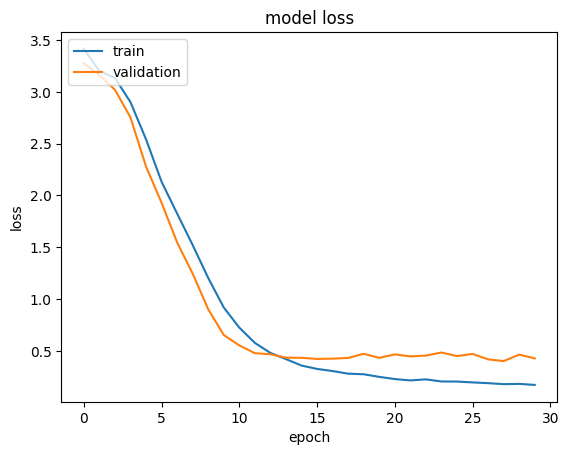
\includegraphics[width = 0.8\linewidth]{loss.png}
\caption{Plot of Model Loss on Train and Validation Datasets}
\label{fig:loss}
\end{figure}

\begin{figure}[!tbhp]
\centering
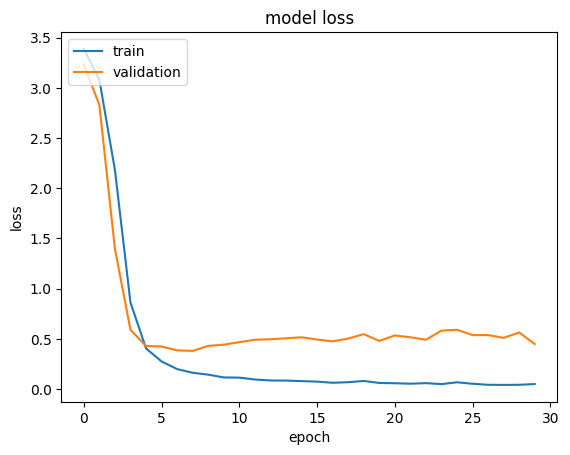
\includegraphics[width = 0.8\linewidth]{loss_d.png}
\caption{Plot of Model Loss on Train and Validation Datasets after removing the dropouts}
\label{fig:lossd}
\end{figure}



\end{document}





